\documentclass[10pt,a4paper]{article}
\usepackage[T1]{fontenc}
\usepackage{times}
\usepackage[pdftex]{graphicx}
\usepackage{etc14}

\begin{document}

\title{Growth and collapse of a finite patch of stratified turbulence}

\authors{\underline{Zachary J. Taylor}$^1$, Alex Liberzon $^1$, Peter J. Diamessis $^2$, \& Roi Gurka $^3$}

\affiliations{$^1$School of Mechanical Engineering, Tel Aviv University, Tel Aviv, Israel\\
$^2$School of Civil and Environmental Engineering, Cornell University, Ithaca, NY, USA\\
$^3$Department of Mechanical Engineering, Ben-Gurion University, Beer-Sheva, Israel\\}
\maketitle
\newcommand{\unit}[1]{\ensuremath{\, \mathrm{\hspace{0.5mm}#1}}}

\begin{summary}
Mixing across lines of constant density is one of the most important aspects of ocean turbulence.  In the current study, experiments have been performed on a finite patch of turbulence in stable stratification.  A finite grid is vertically oscillated to create the three-dimensional patch of turbulence and measurements are made during the growth and collapse of the patch.  The growth of the patch is limited at approximately the same point as previous studies on one- and two-dimensional patches.  Previous studies have suggested that the mixing characteristics of the patch are determined by the interaction between the turbulent flow and the ambient flow near the patch boundaries.  The spatial data obtained in the current study are analysed in the context of the turbulent flow field near the boundaries of the patch.    
\end{summary}

\section{Introduction}

Oceanic observations have suggested that there exist spatially sporadic patches of high intensity turbulence within the pycnocline \cite{Nasmyth1970}.  The pycnocline exists below the mixed surface layer and extends downwards encompassing the ocean's greatest density gradient.  These sporadic patches of high intensity turbulence represent a significant component of the overall mixing in the ocean.  To investigate how a patch of turbulence evolves in the oceanic pycnocline, Fernando \cite{Fernando1988} created a one-dimensional patch by vertically oscillating a grid in a tank with a stable linear stratification.  He found that the initial growth of the patch was negligibly affected by the restoring buoyancy forces until approximately $Nt\approx 4$.  Here, time is non-dimensionalized by the Brunt-V\"ais\"al\"a frequency $N$ defined by, $N^2=-(g/\rho_0)(d\rho/dz)$ where $g$ is the acceleration due to gravity, $\rho_0$ is a reference density, and $d\rho/dz$ is the density gradient.  In a later study, de Silva and Fernando \cite{Silva1998} performed experiments on a two-dimensional patch allowing for growth in the lateral in addition to the vertical direction.  In their study, they observed a similar arresting of vertical growth as in the one-dimensional case and characterized the lateral advancement of the intrusion formed by the patch collapse.
\\
\\
Previous data within the patch have been obtained through point measurements.  These data have highlighted the importance of the interaction between the ambient fluid and that within the patch \cite{Silva1998} near the patch boundaries.  The current study uses data with high spatial resolution to assess the turbulence within the patch.  In addition to the description of the turbulent flow field within the patch, part of the focus of the current study will be to use the high spatial resolution to characterize turbulent mixing near the patch boundaries.  

\section{Details of the experiments}

Experiments have been performed by vertically oscillating a grid in a glass aquarium having a cross-section of $20\times50\unit{cm^2}$ and a depth of $20\unit{cm}$.  The grid has a mesh size of $1\unit{cm}$ and a bar-to-mesh ratio of 1:5 (equivalent solidity is 30.6\%).  The grid is finite in both directions -- in the sense that it is far from the walls -- with dimensions of $6\times6\unit{cm^2}$.  The stroke of the vertical oscillations is $1\unit{cm}$ reaching a maximum frequency of approximately $5\unit{Hz}$.  Because part of our focus is on the initial evolution of the patch, care was taken to minimize any impulse from the start-up of the oscillations by providing a ramp input to the DC motor over the first second.  To create the patch, the grid is forced for 8 seconds including the 1 second ramp start-up.
\\\\
The linear stable stratification is achieved using the free-flow two-tank method \cite{Economidou2009}.  Three different solutions are used in these experiments: homogeneous solution (freshwater), salt-stratified solution, and a stratified solution of Epsom salt water and sugar water.  The last of these was employed to have a stratified solution with a constant index-of-refraction \cite{McDougall1979} so that the Particle Image Velocimetry (PIV) measurements would be free of any optical distortions.  In both of the stratified solutions the Brunt-V\"ais\"al\"a frequency was $N=1$.

\section{Results}

Two different measurement techniques have been used to obtain information about the density field and velocity field, respectively.  In order to qualitatively assess the variation in the density field synthetic schlieren measurements \cite{Aguilar2006} have been performed with an example shown during the growth of the patch in Figure \ref{fig:buildup}.  Also in Figure \ref{fig:buildup} are the out-of-plane vorticity contours calculated from the PIV data.  As in the study on one- and two-dimensional patches \cite{Fernando1988,Silva1998} the growth of the patch is slowed in the presence of buoyancy effects at $Nt\approx4$.
\\\\
After $Nt\approx4$ the patch is observed to collapse horizontally as shown by the qualitative density measurements and the vorticity data in Figure \ref{fig:collapse}.  It is observed from both Figures \ref{fig:buildup} and \ref{fig:collapse} that the vorticity field extends quite close to the boundaries in the density field.  However, the distinction between the ambient fluid and the turbulent flow within the patch is clearer from the qualitative density measurements than in the vorticity field.

\begin{figure}
\setlength{\unitlength}{1cm}
\begin{center} 
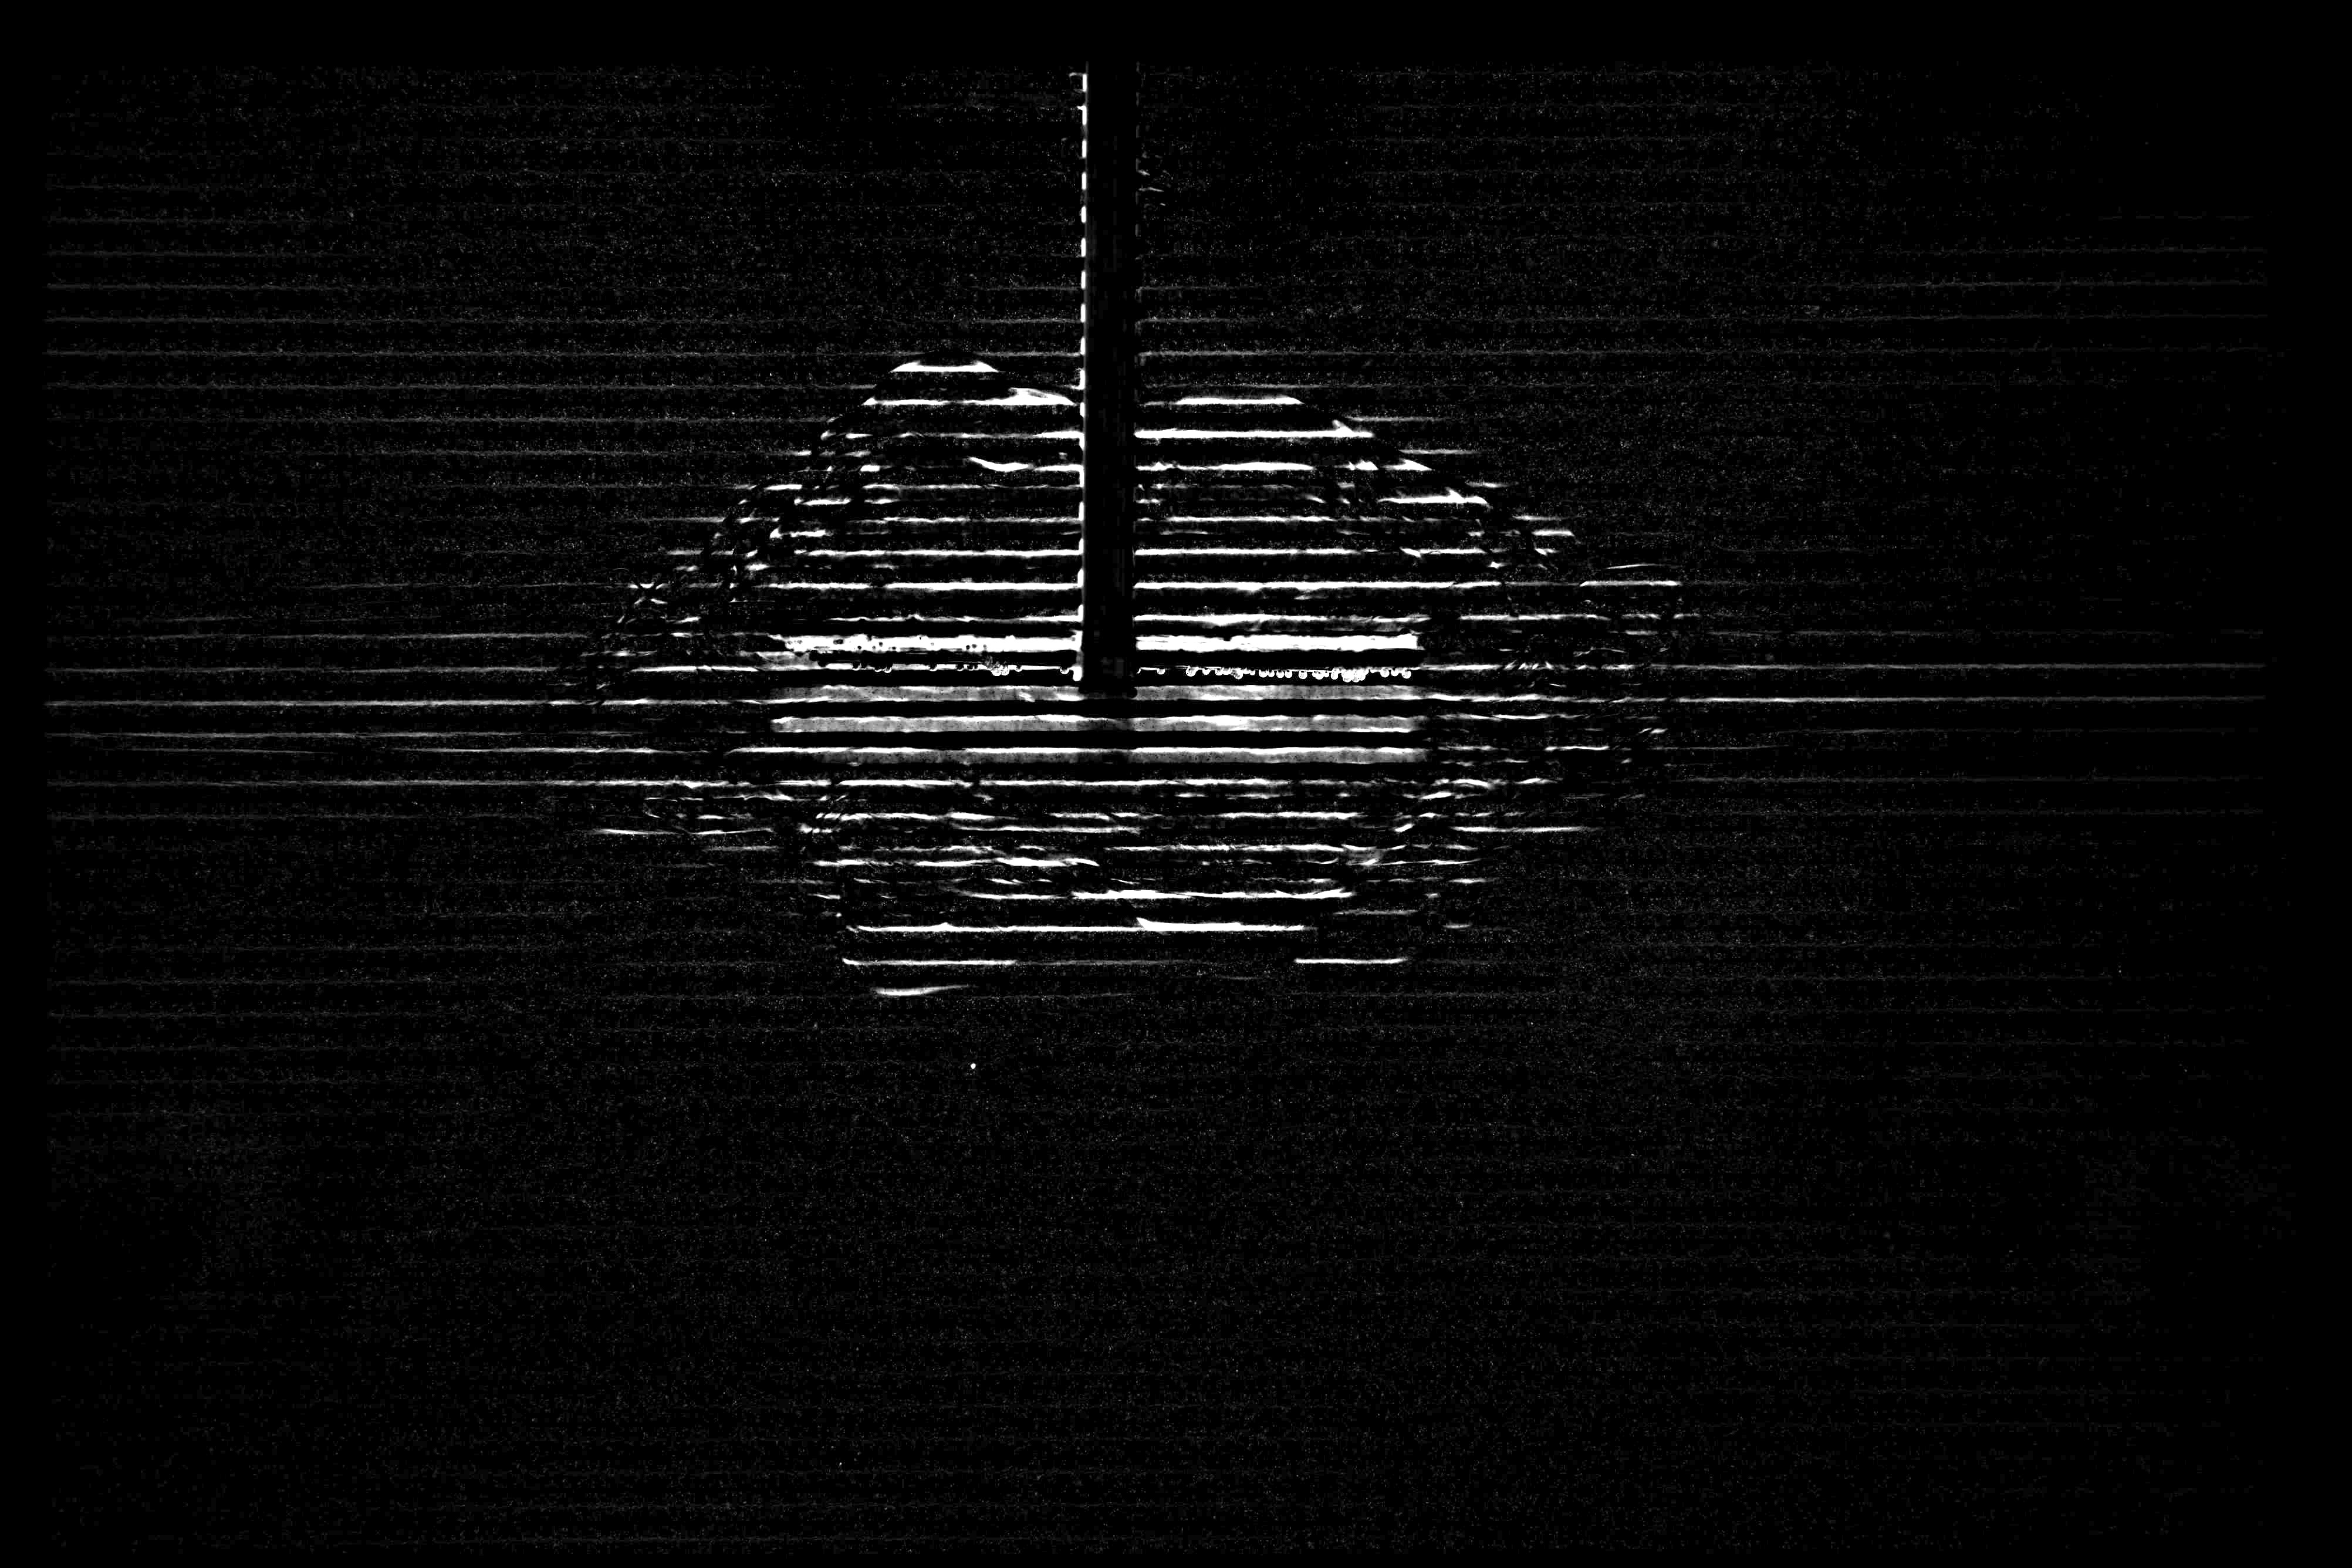
\includegraphics[width=0.3\textwidth]{figures/synthschlieren000137.jpg} \hspace{1cm}
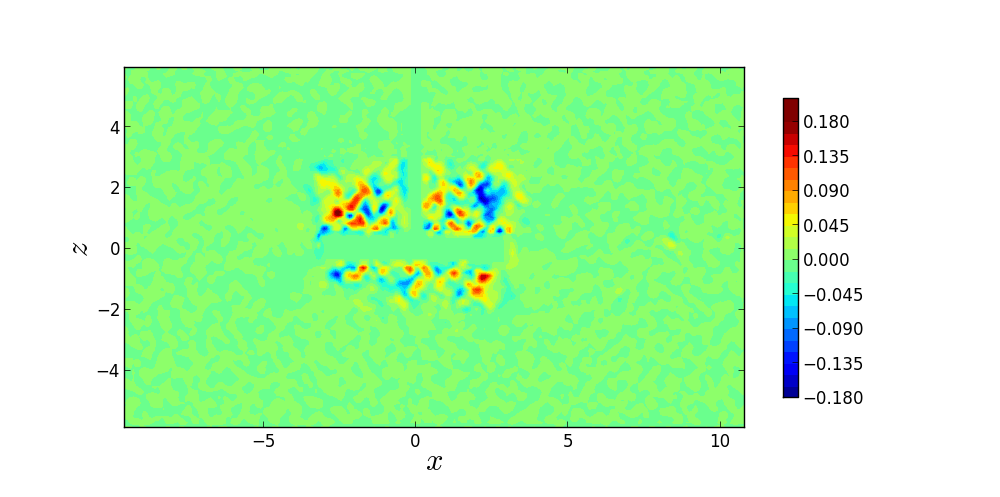
\includegraphics[trim=15mm 5mm 23mm 10mm, clip, width=0.4\textwidth]{figures/buildup.png}
\end{center}
\caption{Measurements during the growth of a turbulent patch.  On the left is a synthetic schlieren image with image subtraction, and on the right is vorticity calculated from instantaneous PIV data.  For the PIV data, the axes have units of centimetres and the colour bar has units of $\mathrm{rad \cdot s^{-1}}$.}
\label{fig:buildup}
\end{figure}

\begin{figure}
\setlength{\unitlength}{1cm}
\begin{center} 
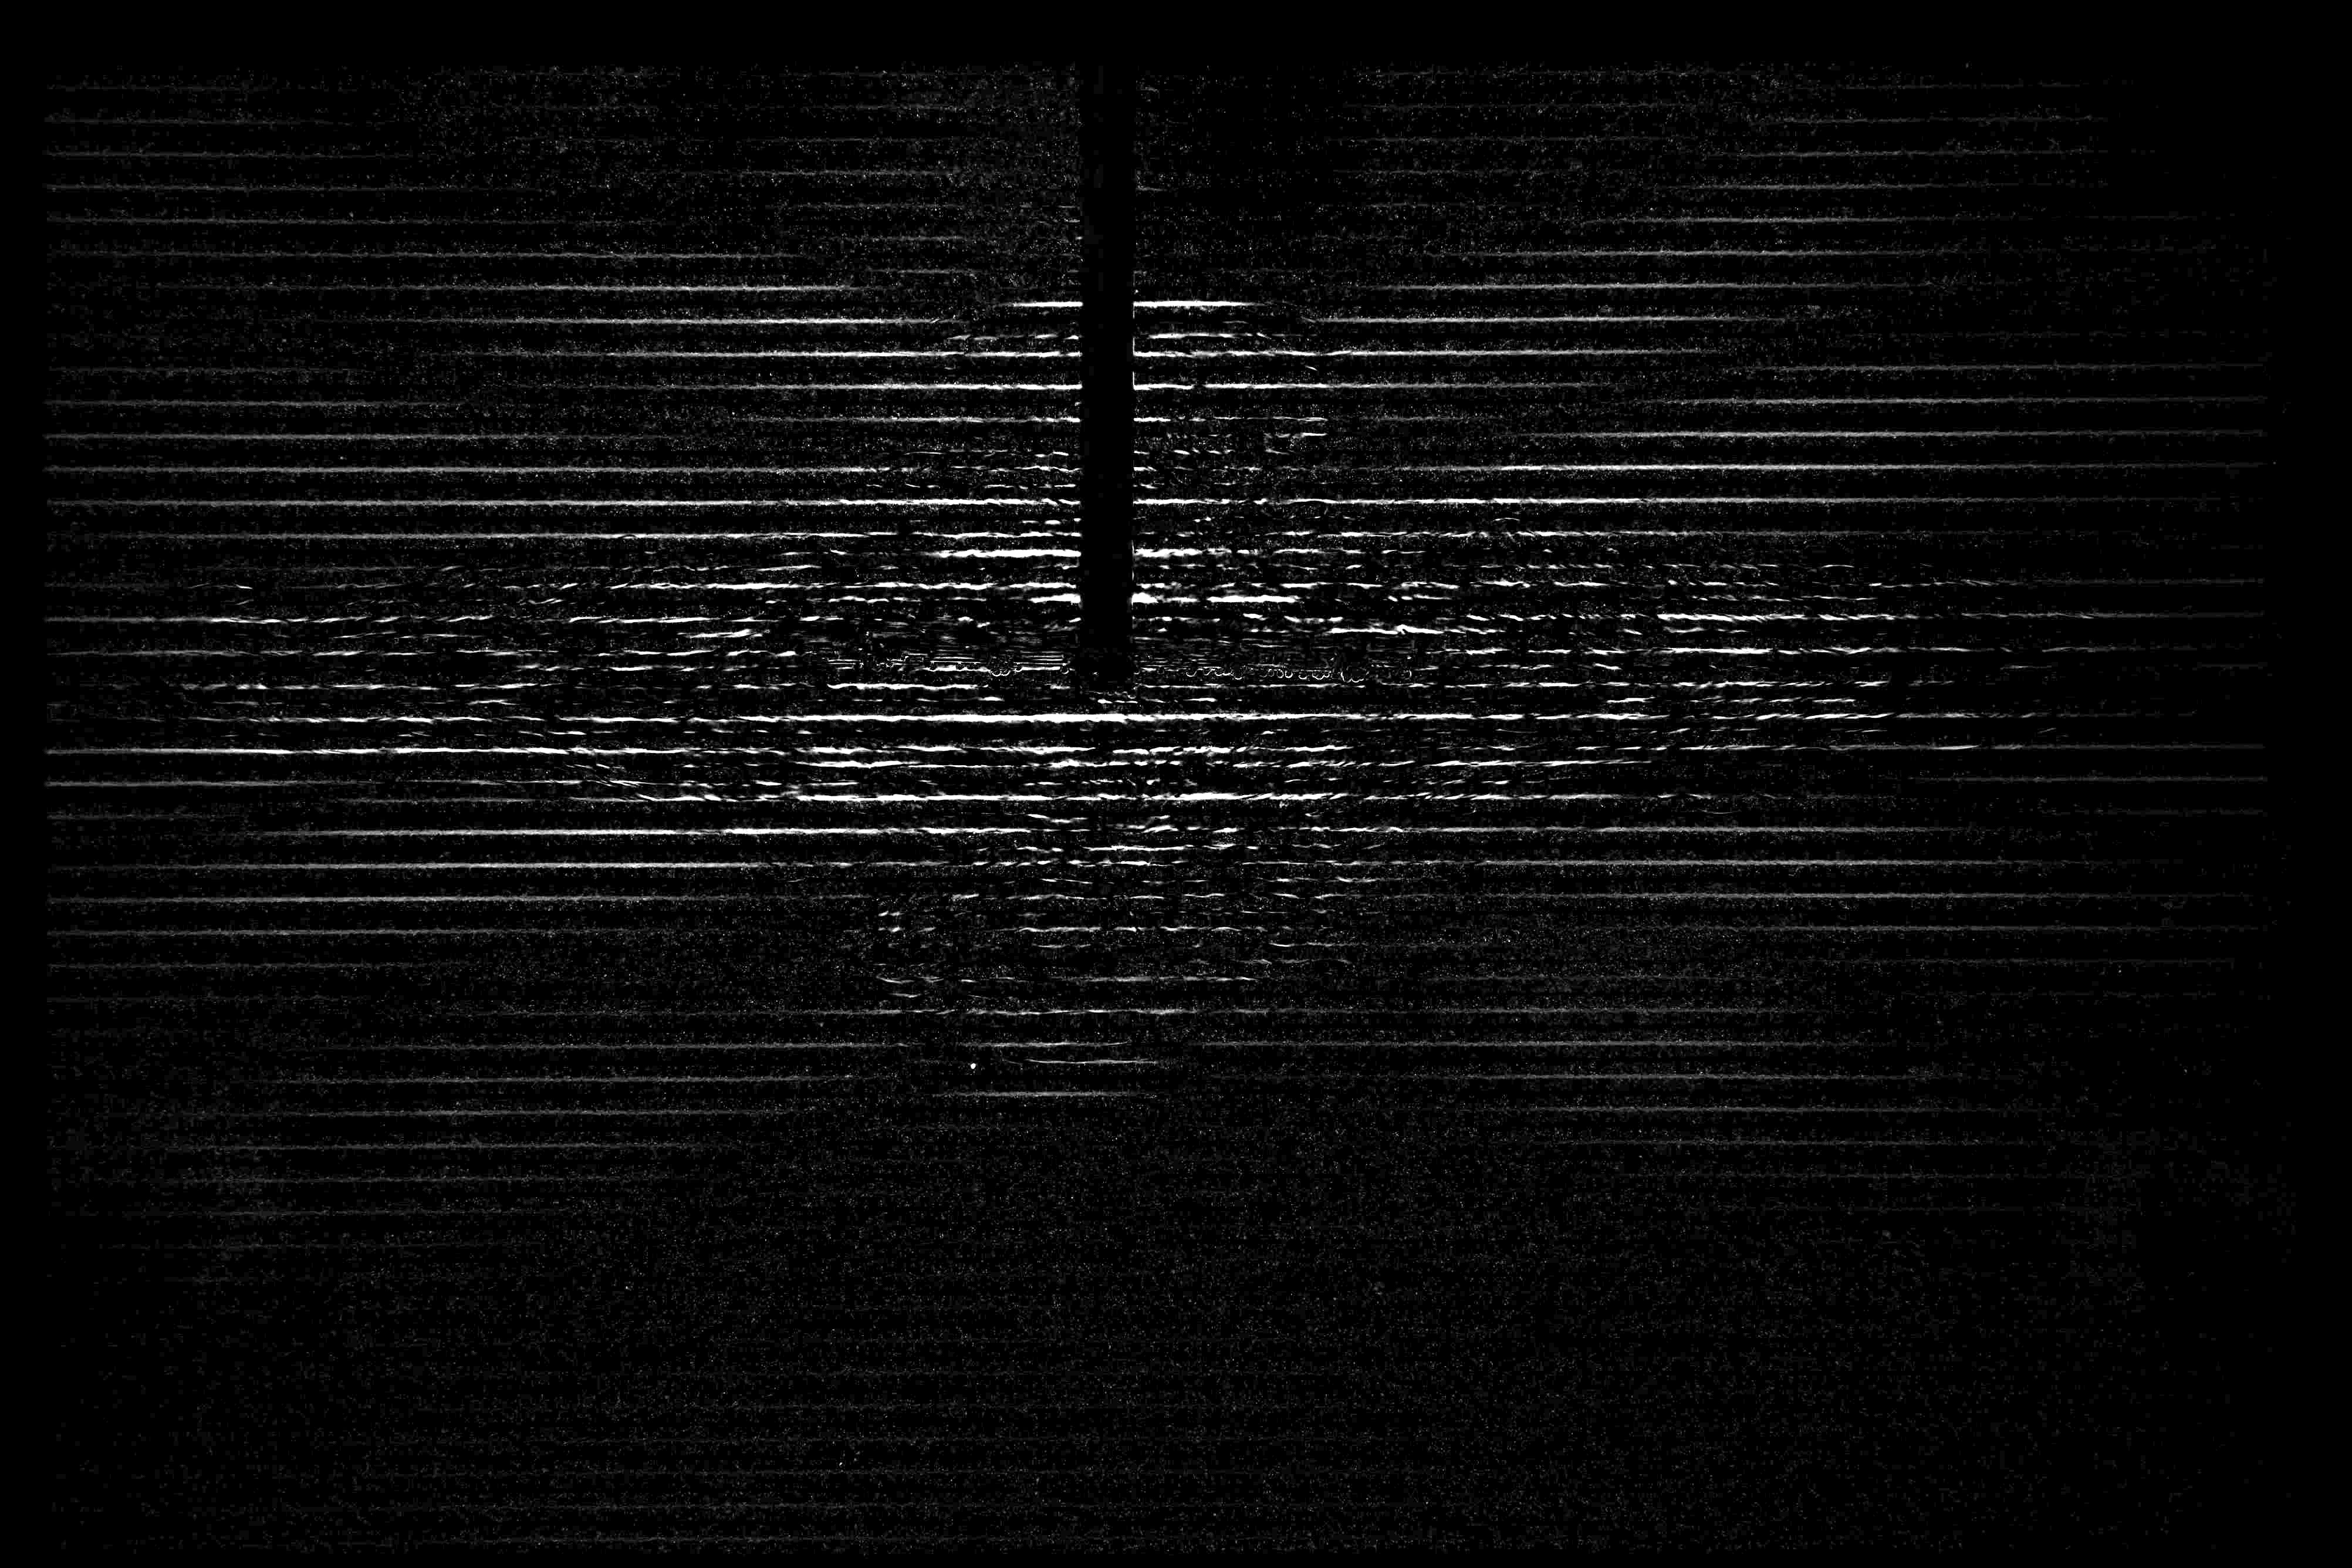
\includegraphics[width=0.3\textwidth]{figures/synthschlieren000150.jpg} \hspace{1cm}
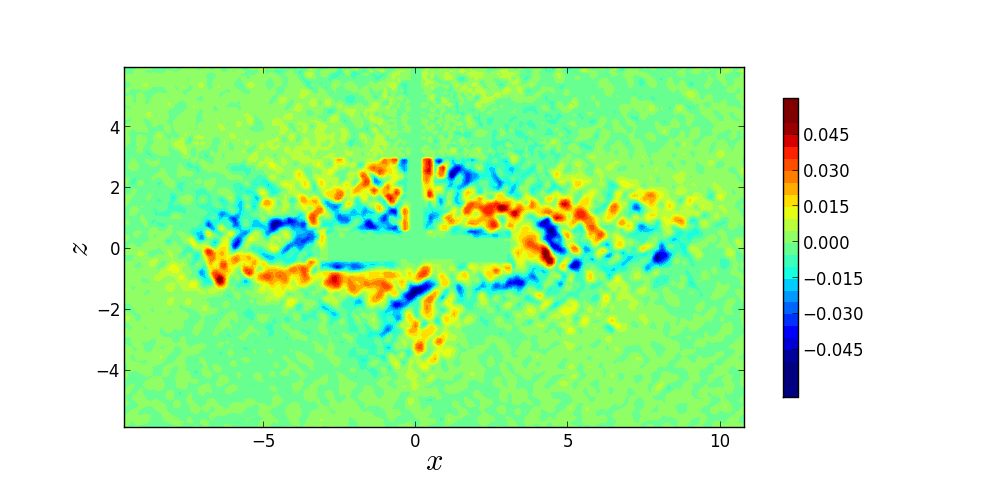
\includegraphics[trim=15mm 5mm 23mm 10mm, clip, width=0.4\textwidth]{figures/collapse.png}
\end{center}
\caption{Measurements during the collapse of a turbulent patch.  On the left is a synthetic schlieren image with image subtraction, and on the right is vorticity calculated from instantaneous PIV data.  For the PIV data, the axes have units of centimetres and the colour bar has units of $\mathrm{rad \cdot s^{-1}}$.}
\label{fig:collapse}
\end{figure}

\section{Conclusion}

Measurements have been performed on a finite turbulent patch in stable stratification.  The dynamics of turbulent patches in stratification are an important part in the overall understanding of oceanic turbulence.  Through PIV measurements and qualitative density measurements it has been shown that the vorticity field extends approximately to the boundaries of the patch in the density field.  However, more in-depth analysis of whether or not these two boundaries coincide will be included for the conference.  Attention will also be paid to the relationship between the density field and the flow field near the patch boundaries in terms of entrainment.  It is this area that previous studies have suggested is crucial to the entrainment of ambient fluid into the patch.  The current set of measurements will offer further insight into how the vorticity structure near the patch boundaries is altered as it increasingly feels the effects of buoyancy and how these changes affect entrainment into the patch.  

\bibliographystyle{plain}
%\bibliography{../../../../research_papers/paperdb,../../../../books/booklist}
\input{bib.bbl}


\end{document}

